\chapter{Fundamentação Teórica}
\label{cap2}



\section{Jogos Eletrônicos}



O primeiro sistema de entretenimento interativo foi construido em 1947, utilizando como base de exibição um tubo de raios catódicos, criado por Thomas Goldsmith Jr. e Estle Ray Mann.
%
Essa criação foi patenteada em janeiro de 1948, datando então o inicio dos jogos eletrônicos~\cite{Adams2014Jan, patents1947Jan}.



O jogo eletrônico, ou entretenimento interativo, é uma atividade intelectual que integra um sistema de regras, na qual utiliza tal sistema a fim de definir seus objetivos ou pontuação por meio de um computador a fim de dispertar alguma emoção ao jogador~\cite{video_game_technologies}.
%
Os jogos eletrônicos são aplicações convencionais, que executam sobre algum sistema operacional ou hardware proprietário.
%
O sistema operacional, hardware ou base de execução da aplicação gráfica define a sua plataforma, \textit{e. g.,} Linux, Windows, PS4, XBox, Web~\cite{adams_1208533}.



Inicialmente os jogos eram implementados de forma simples por conta do hardware limitado dos anos 80.
%
As implementações de jogos para videogames eram desenhadas diretamente para algum hardware proprietário, sem sistema operacional, por muitas vezes sem utilizar comunicação por rede ou memória de disco~\cite{adams_1208533}.
%
Já os jogos de computadores, a qual tinham acesso a rede, eram inviabilizados pelo custo de manutenção de tais serviços~\cite{adams_1208533}.
%
Na década de 80, o videogame Atari foi uma plataforma popular, vendendo 30.000 cópias contra apenas 2.000 cópias do seu concorrente Intellivision~\cite{atari_age}. A sua especificação era:



\begin{itemize}
  \item \ac{cpu} com 1.19 \ac{mhz}
  \item Processador de audio e vídeo dedicado \ac{tia}, permitindo a alteração de 40 x 192 pixels a cada frame usando a tecnologia \ac{ntsc} e 2 canais de som monofônico com 4 bits de intonação e 1 bit de volume.
  \item 128 bytes de memória \ac{RAM}, podendo ser expandido com o cartucho.
  \item Os cartuchos podem ter, no máximo, 4 kB de capacidade.
\end{itemize}



Com o crescente recurso computacional disponível em computadores pessoais e videogames após os anos 90, desenvolvedores criaram novos estilos de jogos que utilizavam a comunicação entre computadores.
%
Jogos como Habitat\footnote{Habitat: \url{http://www.mobygames.com/game/c64/habitat/credits}}, Tibia\footnote{Tibia: \url{http://www.tibia.com/}} e Runescape\footnote{Runescape: \url{https://www.runescape.com}} começam a utilizar, como requisito básico do jogo, a comunicação com a rede.
%
Tais jogos popularizaram os jogos do gênero \ac{mmo}, deixando de ser aplicações locais para ser clientes de um serviço arquitetado na Internet~\cite{adams_1208533, Adams2014Jan}.



\subsection{Árvore de gêneros de jogos eletrônicos}



\begin{figure}[htb!]
\caption{Árvore de gêneros simplificada.}
\label{fig:generos}
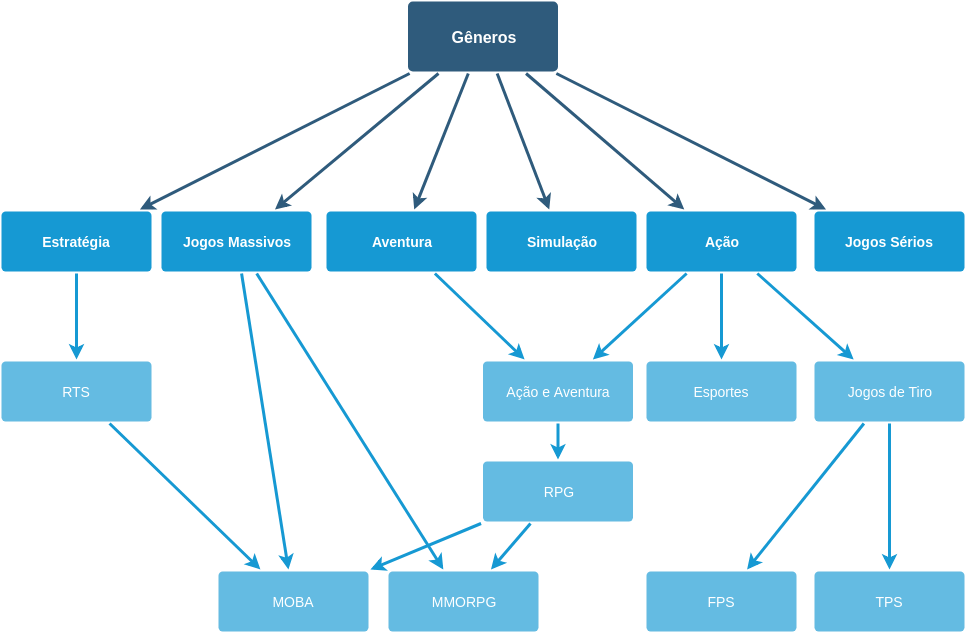
\includegraphics[height=9cm]{img/cap2/generos.png}
\centering

Adaptado de:~\cite{adams_1208533}
\end{figure}



Um gênero de jogo eletrônico é uma categoria específica para agrupar estilos de jogabilidade parecidos.
%
Porém, gêneros não definem definitivamente o conteúdo expresso em algum título, mas sim um desafio comum presente no título analisado~\cite{adams_1208533, video_game_technologies}.
%
Cada gênero de jogo contém várias variações, para uma melhor classificação.
%
A árvore pode ser visualizada pelo diagrama na figura \ref{fig:generos}.



\begin{itemize}
  \item Estratégia
  \item Jogos Massivos
  \item Aventura
  \item Simulação
  \item Ação
  \item Jogos sérios
\end{itemize}


\section{Jogos Massivos}



Jogos \ac{mmorpg} são utilizados como negócio viável e lucrativo, sendo que experiência de jogabilidade na qual o usuário final será submitido é um fator crítico para o sucesso.
%
O mercado de jogos \ac{mmorpg} vem crescendo desde 2012~\cite{new_york_times}, sendo no ano de 2016 um dos mais lucrativos~\cite{statista_2016}.
%
A sua projeção para 2018 é que sejam arrecadados mais de 30 bilhões de dólares americanos com esta categoria de jogos~\cite{statista_2018}, um aumento de 20\% a mais sobre o ano de 2016.



\ac{mmorpg} são jogos de interpretação de papéis massivos, originados dos gêneros \ac{rpg}.
%
A principal característica desse estilo de jogo é a comunicação e representação virtual de um mundo fantasia no qual cada jogador pode interagir com objetos virtuais compartilhados ou tomar ações sobre outros jogadores em tempo real, tendo como principais objetivos a resolução de problemas conforme a sua regra de \textit{design}, o desenvolvimento do personagem e a interação entre os jogadores\cite{video_game_technologies}.
%

Um jogo \ac{mmorpg} é arquitetado em duas partes~\cite{mmo_analytic}:
\begin{itemize}
  \item \textbf{Serviço}: É o macrosserviço que implementa as regras de negócio e requisitos do jogo.
  O serviço disponibiliza uma interface com ações possíveis ao cliente sobre algum protocolo de rede.
  \item \textbf{Cliente}: Cliente é a aplicação que realizará as requisições com a interface do macrosserviço, exibindo o estado de jogo de forma imersiva ao jogador.
\end{itemize}


Um jogo \ac{mmorpg} é arquitetado em duas partes~\cite{mmo_analytic}:
\begin{itemize}
  \item \textbf{Serviço}: É o macrosserviço que implementa as regras de negócio e requisitos do jogo.
  O serviço disponibiliza uma interface com ações possíveis ao cliente sobre algum protocolo de rede.
  \item \textbf{Cliente}: Cliente é a aplicação que realizará as requisições com a interface do macrosserviço, exibindo o estado de jogo de forma imersiva ao jogador.
\end{itemize}

A maioria dos jogos \ac{mmorpg} disponíveis no mercado estão implementados sobre uma arquitetura que executa sobre diversos servidores\cite{stephenclarkewillson2017}, nos quais o desempenho destes servidores influencia tanto na experiência de jogabilidade do usuário final, quanto no custo de manutenção destes serviços~\cite{1417630}.
%
Em especial, o presente trabalho tratará com maiores detalhes as arquiteturas utilizadas no serviço dessa categoria de jogos.

\section{Trabalhos Relacionados}
\label{sec:similares}
